
\chapter{Refactoring Differences Tool}
\section{The aims for the tool}
We want to have views that can have different but equivalent refactoring
This is so that people working on the same project can freely refactor with minimal interference to others
When two people refactor the the code that they are able to hold their own individual refactoring with minimal change when they are merged.
Imagine a situation where you are working jointly on a project with someone else and they refactor the code in order to add some additional functionality.  You also need to refactor the code to do your work but both of the changes are different because they clarify different aspects of the source code. 

At the moment when someone attempts to check-in their changes there is a major conflict.  This is because a refactoring often makes a large amount of global changes to the source code.  One of these changes which is not catered for by current version control systems is the change of order.  The first person to check-in their code will have no issue as the version control system assumes that all the changes are simply a new revision.  When the second person attempts to reconcile their view there is the possibility of having many conflicts.  A lot of these conflicts will be with refactored code which although works the same has a different structure.

Often a new project or sub-project is set-up in a new branch. If there is some refactoring before any changes are made when the code is re-merged with the original project (often called the trunk project) both the changes and the refactored code are checked in.

\begin{center}
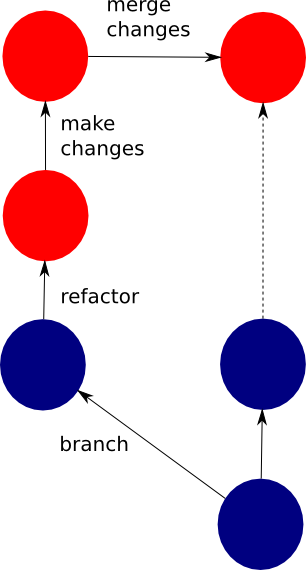
\includegraphics[scale=0.5]{refactorCheckIn}
\end{center}

When there is a large change on a separate branch it could be the case that there are multiple check-ins to keep other parts up to date and ensure that there is not too much divergence.  Currently if you have a project where there are periodic check-ins for each development milestone there will be a large impact each time there is a commit. This is because the refactoring for the large refactored project is imposed upon the repository each time it is checked in.   

% example

% find an example of a workplace situation where refactoring interferes with 
% others

to have less merge conflicts when merging code 

to better be able to detect differences

We want to have views that can have different but equivalent refactoring
This is so that people working on the same project can freely refactor with minimal interference to others

\section{What the tool does}
The tool that has been written not only examines the text differences between two files but also any Java differences. In order to resolve some of the limitations with JDime and the text only merge in GIT information about which line numbers are retained after the first text merge.  In JDime these are ignored and the AST is relied upon to hold all the information.  The change set has been taken from the original GIT based diff contains the start and end of the change in both files and what type of change it is (insert delete or modify).  By reusing these line numbers it is possible to figure out which AST items these changes affect. This is done loading the file into the JastAddJ parser to get an AST tree. The line numbers for each item in the tree are then comparing line numbers from the change

% insert diagram of how it finds the asts that are within the change set
% 
% enhamnces git by adding moves and to a limited extent copies and renames
\section{How the tool works}
\section{How it works}

The refactoring difference tool first works out which text has changed using the same method as git.
The change sets found in using the git histogram comparison are then evaluated.
The reason for this is that some of the items of text could be in a differing order but still be a valid Java program

Comment and white-space are also examined as they could give some indication of where code has been moved from or too

 
\section{Design decisions}
% comments
% whitespace
% the drill down using line numbers
% comparing ASTs
% the matcher and how using a score works
% finding the best match
% 
% why does it do it for the whole repository
% 
% 
% note: we might want to use some literate programming here
\section{Limitations of the tool}
% because it drills down only on the changes it is harder to investigate any 
% change that has causes side effects in unchanged code.  It is not often that 
% a side effect will be purposely placed in the code as it reflects bad design 
% decisions.  This may however be an issue with bugs


 







